\documentclass{beamer}
\usetheme{Boadilla}
\usepackage{hyperref}
\usepackage{graphicx}
\usepackage{multimedia}
\usepackage{fancyvrb}
\usepackage{multicol}
\usepackage{optparams}
\usepackage{adjustbox}
\usepackage{tikz}
\usetikzlibrary{shapes,positioning}
\newcommand{\foo}{\hspace{-2.3pt}$\bullet$ \hspace{5pt}}
\usepackage{subfig}
\usepackage[backend=biber,authordate]{biblatex-chicago}
\addbibresource{citations.bib}
\usepackage{pgfpages}
\usepackage{xcolor}
\definecolor{ao(english)}{rgb}{0.0, 0.5, 0.0}
\definecolor{burgundy}{rgb}{0.5, 0.0, 0.13}
%\setbeameroption{show notes}
\setbeameroption{show notes on second screen=right}
%\setbeameroption{hide notes}

\def\footshortciteintern[#1][#2]#3{%
\ifx#1\empty 
% Nur Autor
\footnote{\citeauthor{#3}, \citeyear{#3}.}
\else
\ifx#2\empty
% Autor und Seite
\footnote{\citeauthor{#3}, \citeyear{#3}, #1.}
\else
% Autor, Seite und vgl.
\expandafter  
\footnote{\citeauthor{#3}, \citetitle{#3}, \citeyear{#3}, \citeurl{#3}.}
\fi
\fi
}
\newcommand*\footshortcite{%
\optparams{\footshortciteintern}{[\empty][\empty]}
}
\newcommand*\footmediumcite{%
\optparams{\footshortciteintern}{[][]}
}

\title{State-of-the-art Beat Tracking}
\author{Sevag Hanssian}
\date{March 30, 2021}
\institute{MUMT 621, Winter 2021}
\setbeamertemplate{navigation symbols}{}

\begin{document}

\begin{frame}
\maketitle
\end{frame}

\begin{frame}
	\frametitle{madmom}
	madmom is an open-source Python MIR library from the Institute of Computational Perception at the Johannes Kepler University,\footfullcite{madmom} containing implementations of the many beat tracking works of Sebastian B{\"o}ck and colleagues
\end{frame}

\begin{frame}
	\frametitle{State-of-the-art results}
	The RNNBeatProcessor\footfullcite{bock1} $\rightarrow$ DBNBeatTrackingProcessor\footfullcite{bock2} algorithm achieved the best results in the last* \textbf{M}usic \textbf{I}nformation \textbf{R}etrieval \textbf{E}valuation e\textbf{X}change audio beat tracking challenge\footnote{\url{https://www.music-ir.org/mirex/wiki/2019:MIREX2019_Results}}\\\ \\

	*: 2020 did not include beat tracking submissions
\end{frame}

\begin{frame}
	\frametitle{State-of-the-art results}
	\begin{figure}
		\subfloat[SMC (Sound and Music Computing at University of Porto) dataset results]{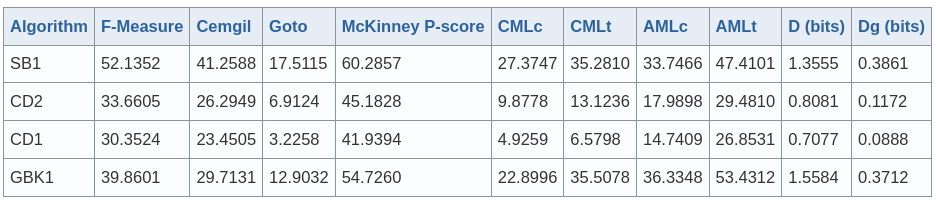
\includegraphics[width=12cm]{./smc.png}}\\
		\vspace{0.1em}
		\subfloat[MAZ (Chopin Mazurka) dataset results]{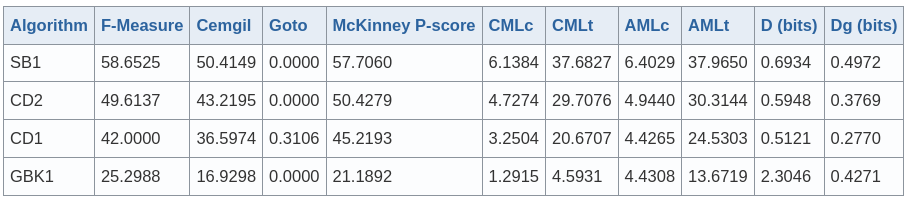
\includegraphics[width=12cm]{./maz.png}}
		\caption{MIREX 2019 audio beat tracking results}
	\end{figure}
\end{frame}

\begin{frame}
	\frametitle{Step 1: RNNBeatProcessor}
	Traditional beat tracking algorithms use onsets, or the beginning of musical events,\footfullcite{onsets} as ``potential beats,'' upon which further post-processing is applied to get beat locations\footfullcite{ellis, goto, btrack}\\\ \\
	The first algorithm, the RNNBeatProcessor\footcite{bock1}, replaces traditional onset detection with a bidirectional Long Short-Term Memory (BLSTM) recurrent neural network to output frame-by-frame beat activations
\end{frame}

\begin{frame}
	\frametitle{BLSTM}
	\textcite{bock1}'s justification for using BLSTM architecture:
	\begin{itemize}
		\item
			Most basic approach of neural networks is the multilayer perceptron (MLP) forming a feed forward (causal) neural network (FNN)
		\item
			Cyclic connections form a recurrent neural network (RNN), which can use past values but suffers from the vanishing gradient problem
		\item
			Long Short-Term Memory (LSTM) solves this problem. If the past \textit{and} future of input are both important, Bidirectional LSTMs add a new layer presented to the network in reverse temporal order
	\end{itemize}
\end{frame}

\note{
	\begin{itemize}
		\item
			strictly causal network, where the output is calculated directly from the input values
		\item
			inputs decaying or blowing up exponentially over time is called the vanishing gradient problem
	\end{itemize}
}

\begin{frame}
	\frametitle{Step 1: RNNBeatProcessor}
	\begin{itemize}
		\item
			Originates from BLSTM onset detection algorithm\footfullcite{rnnonset}
		\item
			Modified to ``suit the needs for audio beat detection by modifying the input representation and adding an advanced peak detection stage''\footcite{bock1}
	\end{itemize}
	\begin{figure}
		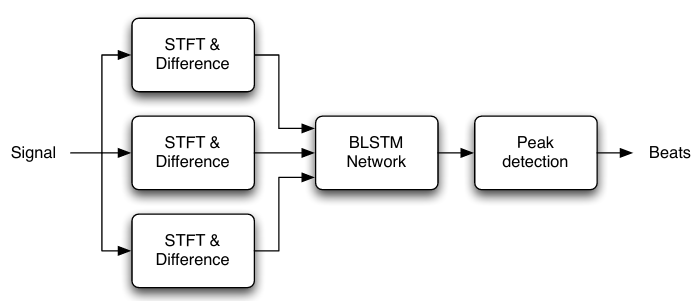
\includegraphics[height=3.5cm]{./rnnbeat.png}
		\caption{RNNBeatProcessor architecture}
	\end{figure}
\end{frame}

\begin{frame}
	\frametitle{Step 2: DBNBeatTrackingProcessor}
	DBNBeatTrackingProcessor:\footfullcite{bock3}
	\begin{itemize}
		\item
			Use \textcite{bock1}'s RNNBeatProcessor with multiple RNNs for different, heterogenous music styles
		\item
			Add an additional dynamic Bayesian network stage\footfullcite{whiteley} which jointly infers the tempo and the beat phase from the beat activations of the RNN stage
		\item
			More efficient implementation of the DBN proposed by \textcite{bock2}
	\end{itemize}
\end{frame}

\begin{frame}
	\frametitle{Step 2: DBNBeatTrackingProcessor}
	\begin{figure}
		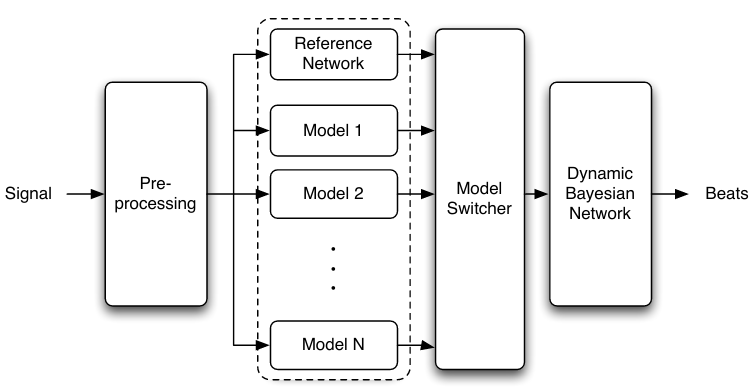
\includegraphics[height=5cm]{./multirnn.png}
		\caption{Multi-model RNN + DBN architecture}
	\end{figure}
\end{frame}

\begin{frame}
	\frametitle{Bar-pointer model}
	Popular model that jointly models tempo and bar position, called the \textit{bar pointer model}\footshortcite{whiteley} is inefficient: ``these algorithms share the problem of a high space and time complexity because of the huge state-space in which they perform inference''\footshortcite{bock2}
	\begin{enumerate}
		\item
			Non-linear tempo resolution matching humans
		\item
			Only allow tempo transitions on beat locations
	\end{enumerate}
	\begin{figure}
		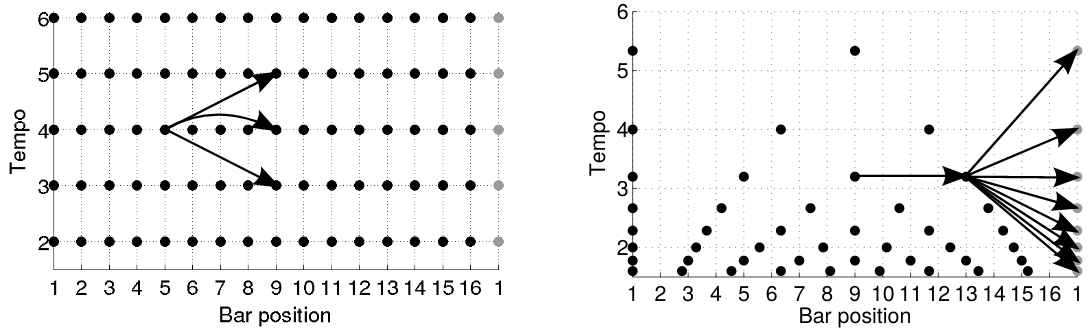
\includegraphics[height=3.25cm]{./efficient.png}
		\caption{More efficient tempo-bar model}
	\end{figure}
\end{frame}

\begin{frame}[fragile]
	\frametitle{Complete example}
	Suggested usage from madmom docs:\footnote{\url{https://madmom.readthedocs.io/en/latest/modules/features/beats.html}}
	\begin{Verbatim}[fontsize=\small]
>>> proc = DBNBeatTrackingProcessor(fps=100)
<madmom.features.beats.DBNBeatTrackingProcessor object at 0x...>
>>> act = RNNBeatProcessor()('tests/data/audio/sample.wav')
>>> proc(act)
array([0.1 , 0.45, 0.8 , 1.12, 1.48, 1.8 , 2.15, 2.49])
	\end{Verbatim}
\end{frame}

\begin{frame}
	\adjustbox{valign=c}{{\usebeamerfont{frametitle}\usebeamercolor[fg]{frametitle}Conclusion}}\hfill
	\adjustbox{valign=c}{
	\newcounter{year}
	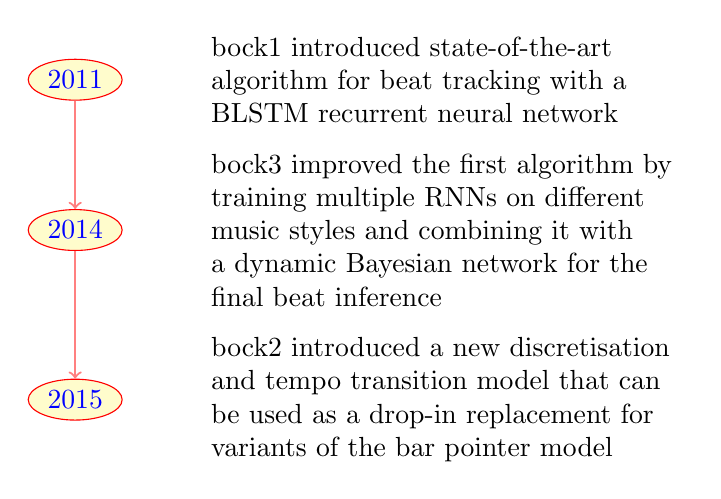
\begin{tikzpicture}[yscale=0.5,%
		   year/.style={draw=red,text=blue,fill=yellow!20,shape=ellipse,inner sep=2pt},
		   description/.style={rectangle,align=left,text width=60mm,anchor=west},
		   timeline/.style={->,thick,red!50}]

	    \foreach \year/\desc [count=\y] in {%
		    2011/\textcite{bock1} introduced state-of-the-art algorithm for beat tracking with a BLSTM recurrent neural network,%
		    2014/\textcite{bock3} improved the first algorithm by training multiple RNNs on different music styles and combining it with a dynamic Bayesian network for the final beat inference,%
		    2015/\textcite{bock2} introduced a new discretisation and tempo transition model that can be used as a drop-in replacement for variants of the bar pointer model%
	       } { \ifnum\y=1 \node[description](\y){\desc};
		   \else\node[description,below=1ex of \z](\y){\desc};
		   \fi
		   \node[year](y-\y) [left=of \y] {\year};
		   \ifnum\y>1\draw[timeline] (y-\z)-- (y-\y);\fi
		   \global\let\z=\y% for drawing from last node
	       }

	\end{tikzpicture}
	}
\end{frame}

\end{document}
